\section{Creating a metamodel}
\subsection{Metamodeling introduction}

The first question you might be asking yourself is, what is metamodeling ?

Metamodeling can be described as creating the model of a model. That means defining abstract rules and structures an instance of such a metamodel has to fulfill\footnote{See Sprinkle, Rumpe et. Al 2014 }.\newline

For a basic introduction into metamodeling and graph transformation see\footnote{\href{https://www.cs.le.ac.uk/people/rh122/papers/2006/Hec06Nutshell.pdf}{Graph Transformation in a Nutshell}}.

\subsection{Adding the eMoflon toolbar}

Now it is time to get to know the functionalities of eMoflon. First, you should add the \textbf{eMoflon toolbar} to your \textbf{Eclipse} as shown in the chart below.\newline Look for the \textit\textsf{Window} tab in the left top corner and press:\newline

\centering
→ \textit{\textsf{Window}} →
\textit{\textsf{Perspective}} → \textit{\textsf{Open Perspective}} → \textit{\textsf{Other}}
\newline

\raggedright
Then open the \textbf{eMoflon toolbar icon} which is highlighted via the red square in the chart below:\newline\newline
\begin{figure}[h]
    \centering
    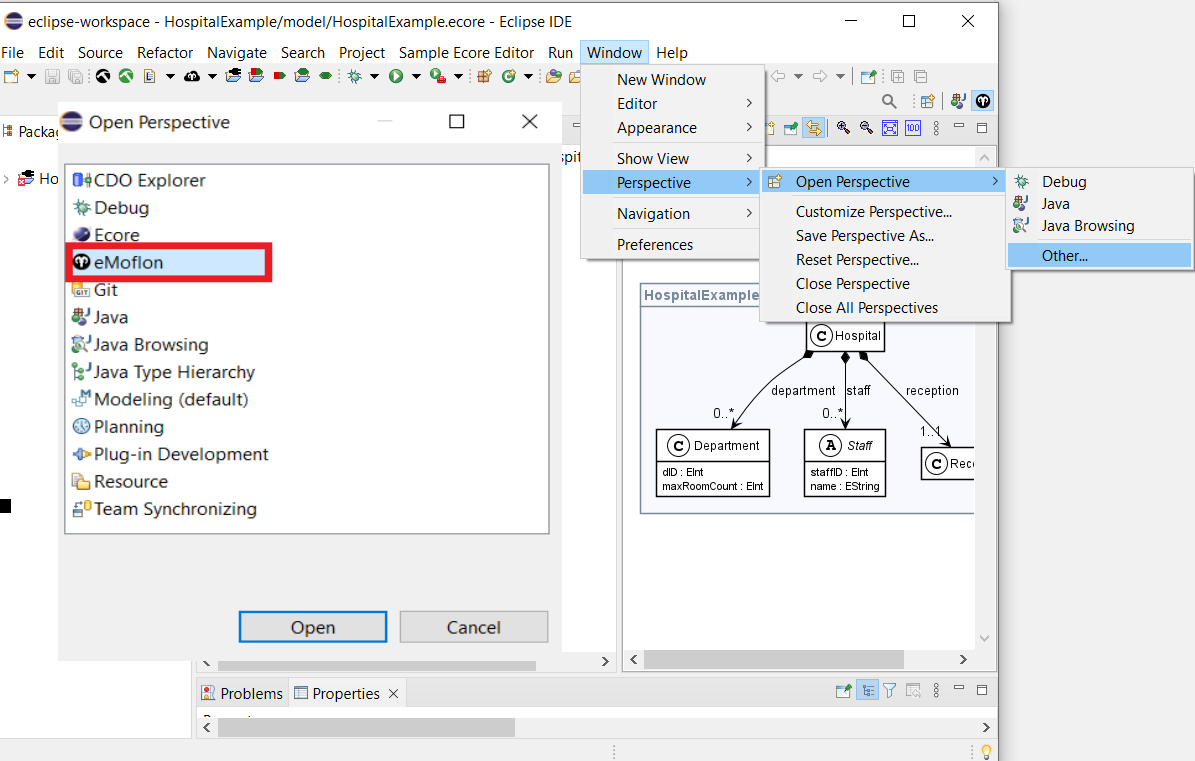
\includegraphics[scale=0.4, width =\textwidth]{pictures/add_perspective.png}
    \caption{\centering{Add the eMoflon toolbar icon}}
    \label{add toolbar}
\end{figure}

\clearpage

\textbf{Functions:\newline}

\begin{figure}[h]
    \centering
    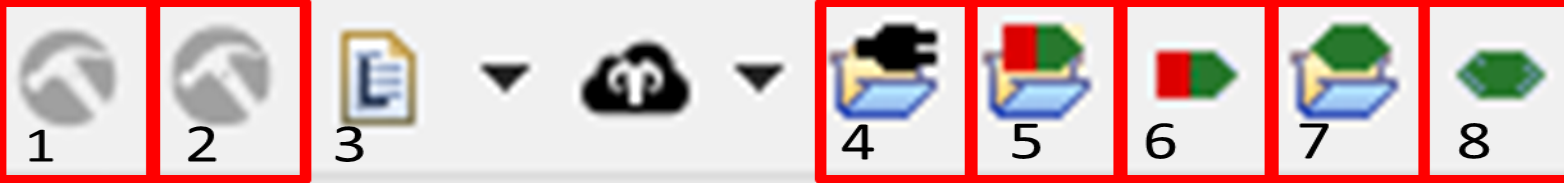
\includegraphics[scale=0.25]{pictures/toolbar_eMoflon.png}
    \caption{\centering{This is how the eMoflon perspective should look like}}
    \label{toolbar}
\end{figure}

Let us take a look at the functions we will need throughout this tutorial:

\begin{enumerate}
\item Clicking this button will \textbf{build} the selected projects \textbf{fully}.
\label{item:0}

\item Clicking this button will \textbf{build} the selected projects \textbf{incrementally}.

\item Clicking this will show you the \textbf{logging configuration} of the eMoflon Console.

\item
\label{item:1}
The folder with the plug \textbf{creates a new eMoflon project}.

\item
\label{item:2}The folder with the green and red arrow \textbf{creates a new graph transformation project}.
\item The green and red arrow \textbf{creates} a simple graph \textbf{transformation file}.
\item 
\label{item:3}The folder with the green trapezoid is used for \textbf{creating triple grammar graph projects}.
\item \label{tgg_rule} The green trapezoid button \textbf{creates} a single \textbf{triple grammar graph file}. 
\end{enumerate}

\clearpage

\subsection{Creating a new EMF project}

First of all we have to create a new \textbf{metamodel}. Click on \textbf{button 4} to create a new \textbf{\textsf{eMoflon EMF Project}} and choose a new name for your project.

For this tutorial we are going to create a scenario which models a hospital and its administration. This is supposed to show you the basic functions of eMoflon::IBeX.\newline You should \textbf{stick to the naming conventions} we are using, since inconsistent names may lead to errors later !\newline

\centering
→ Please select \textit{\textsf{Generate default ecore file}}\newline

\raggedright
Please give the project the name \textit{\textsf{HospitalExample}} as shown in the chart below. After you have pressed the \textit{\textsf{finish}} button a new file should appear in the model folder. If you cannot see it, try to refresh the folder.\newline

\begin{figure}[h]
    \centering
    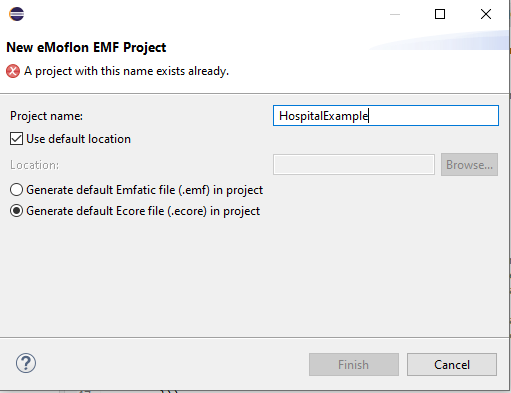
\includegraphics[scale=0.7]{pictures/project_creation.png}
    \caption{\centering{Creation of a new EMF project}}
    \label{project creation}
\end{figure}
\clearpage
\subsection{Filling the model with content}

 The chart below provides a UML-based visualization of the finished model you will create throughout this part of the tutorial. If you are not sure whether your model is correct, you can use this as a comparison:\newline
 
\begin{figure}[h]
    \centering
    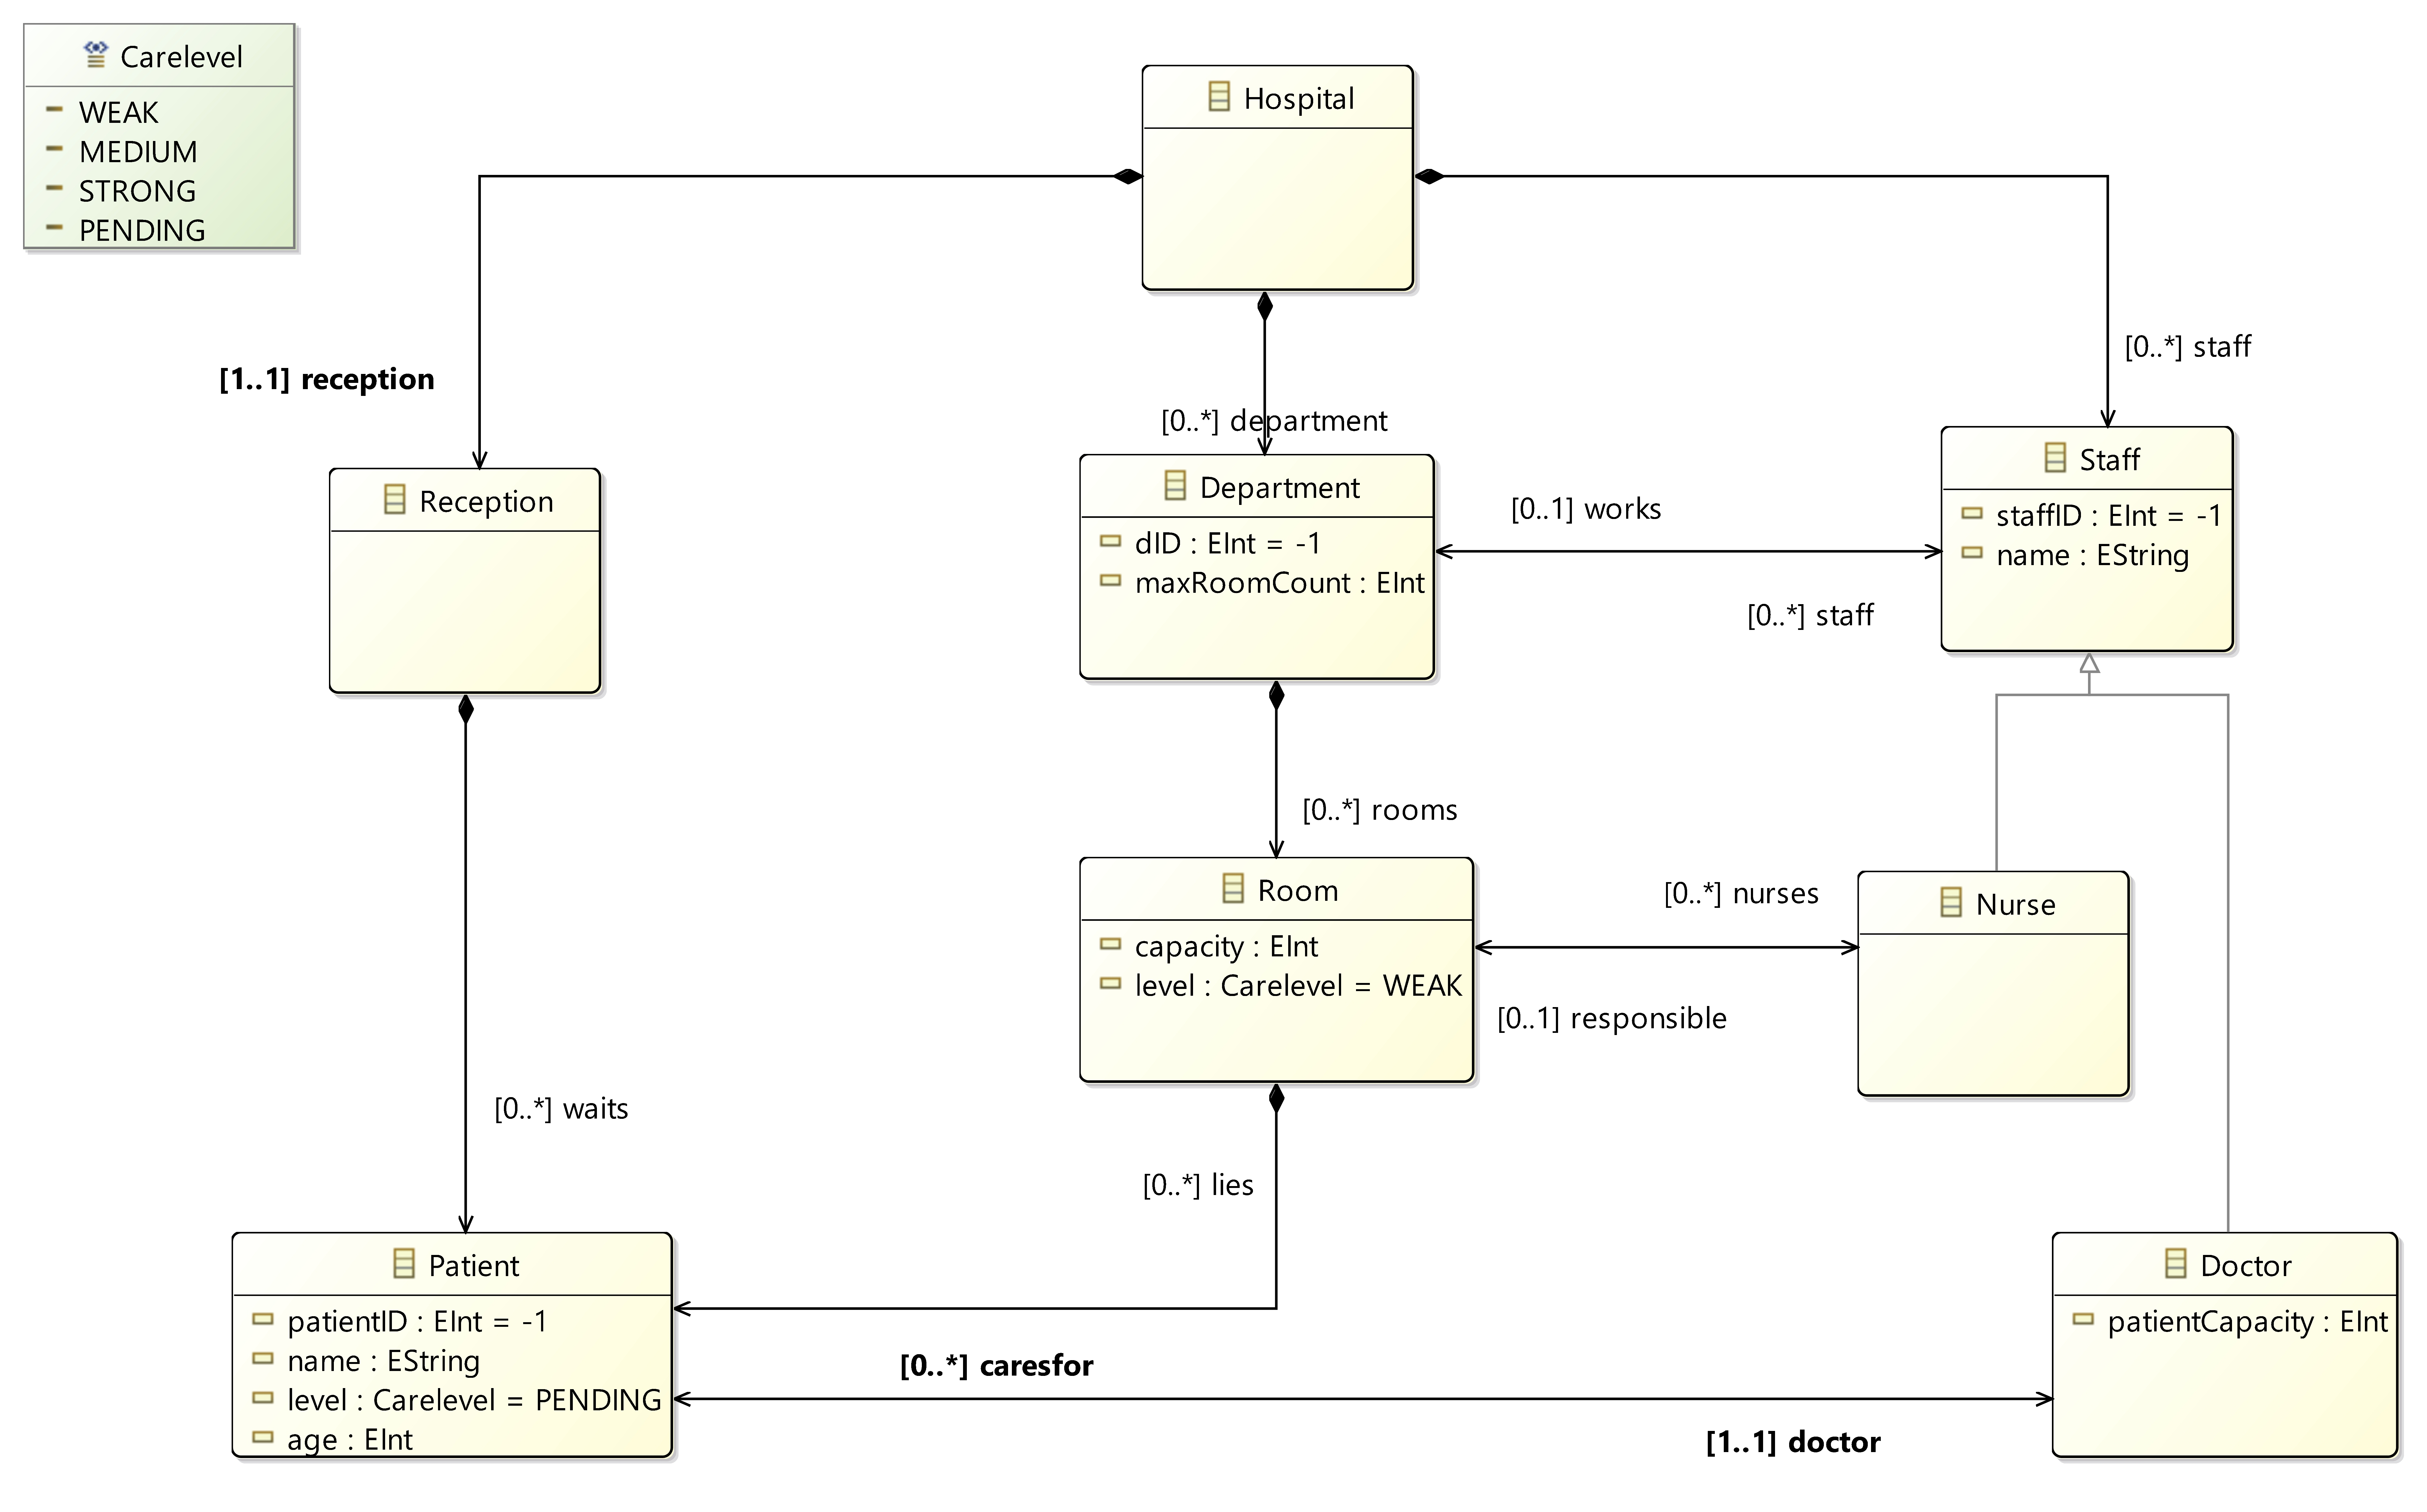
\includegraphics[scale=0.9, width= \textwidth]{pictures/model_finished.jpg}
    \caption{\centering{Complete model}}
    \label{goal model}
\end{figure}

\textbf{Note:}

To visualize you current model left-click on \textit{\textsf{HospitalExample}} and look at the \textbf{PlantUML tab} in the top right corner. This will look a bit different than this UML chart, but should be equal in regard to its content.

\clearpage

The first class we need for our tutorial is the hospital itself. To create the \textbf{Hospital class}, you need to \textbf{right-click} on the \textit{\textsf{HospitalExample}} package and select \textbf{EClass} in the drop-down menu as a new child of the metamodel.\newline

\begin{figure}[h]
    \centering
    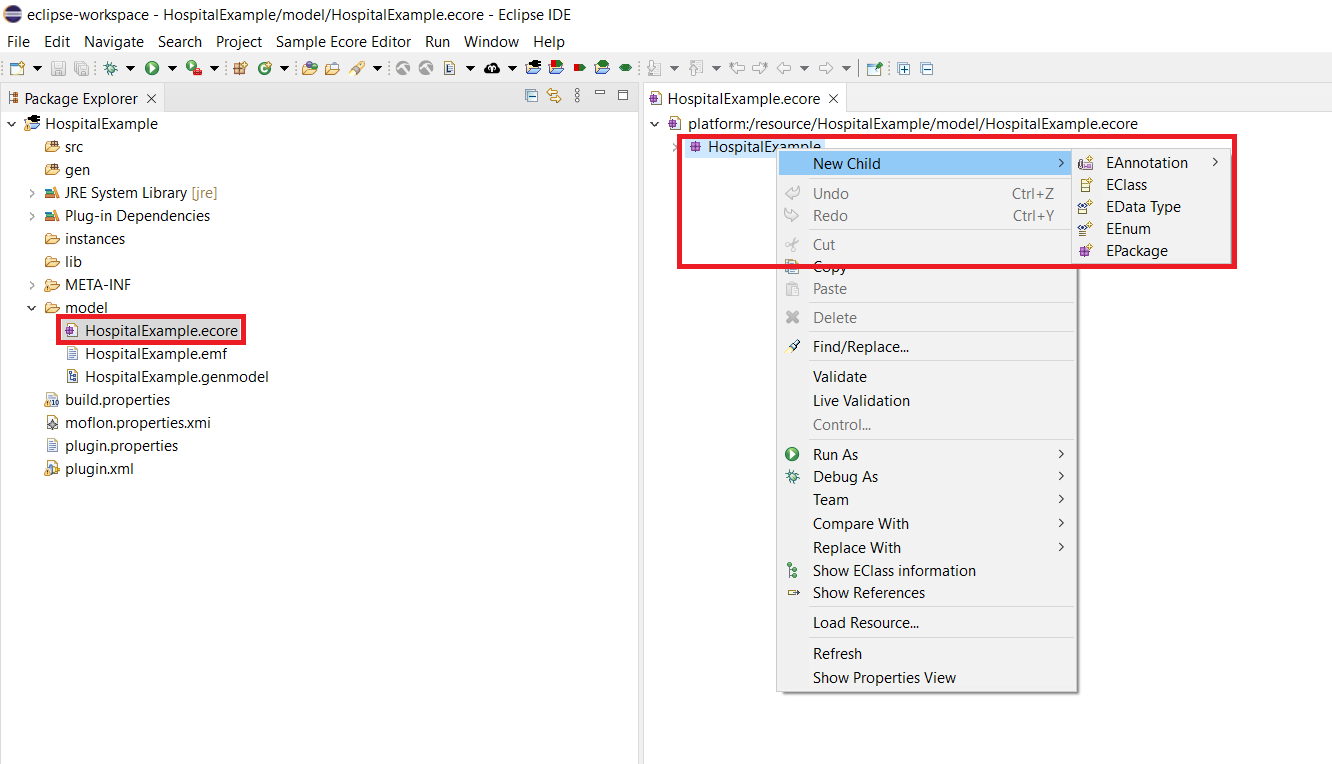
\includegraphics[scale=0.5, width= \textwidth]{pictures/new_child.png}
    \caption{\centering{Create Hospital class as child of the metamodel}}
    \label{project creation}
\end{figure}

As you can see, it is also possible to create an \textbf{enumeration}, a \textbf{data type}, and \textbf{other packages} to split up your project.\newline You may have noticed that every option begins with a capital "E". This is merely a \textbf{naming convention} used in EMF and it will be also used for things such as variable types. For example, a variable of the type of integer has to be defined as "EInt".\newline

After you have created the Hospital, you can define its \textbf{properties} in the \textsf{\textit{properties}} window. If you cannot see the properties window, right-click on the \textit{\textsf{Hospital}} child you have just created and select \textit{\textsf{Show Properties View}} on the bottom of the list or \textbf{double left-click} on the child.

Let us name the class accordingly by typing \textit{\textsf{Hospital}} in the name field. All other fields can be left set to their default value.\newline

To fill our Hospital, we start by adding a \textsf{\textit{reception}} class and a \textsf{\textit{department}} class. This is done in the same way as for \textit{\textsf{Hospital}}.\newline

After creating the classes, we have to connect them to our hospital. This can be done by creating a \textbf{new child} in our hospital class. This child is of type \textbf{EReference}.
The properties of a \textbf{reference} offer a large variety of options you can configure but let's keep it simple for now.

To maintain comprehensibility and simplicity in your model \textbf{naming your reference} after the corresponding class or its purpose is recommended.

Hence, we chose the name \textsf{\textit{reception}}.\newline

Furthermore, we also need a \textbf{type} for our reference which can be defined in the \textbf{EType field}, where we select the type \textsf{\textit{Reception}}.\newline

Naturally, a hospital has only one reception, so we have to modify the \textbf{multiplicities} of our references as well. \textbf{Multiplicities} can be configured via the \textsf{"Lower Bound"} and \textsf{"Upper Bound"} options. By changing the \textbf{lower bound} value to \textbf{1} we ensure that our hospital has \textbf{at least one} reception. To avoid having \textbf{more than one} reception in the Hospital you have to set the value for the \textbf{upper bound} to \textbf{1} as well. If you want to model an \textbf{N-multiplicity} you have to set the \textbf{upper bound} to \textbf{-1}.\newline

Please note that it is also possible to change the \textbf{boundaries of attributes}. However, meddling with the attribute boundaries can easily mess up your model. Hence, we advise you to leave the boundaries of attributes as they are by default.\newline

The model depicts the relation between the Hospital and the Department class with a \textbf{rhomb} this means the relationship is a \textbf{containment}. You have to set the value of the \textsf{"Containment"} field to \textsf{true}.\newline

Please create the \textbf{department reference} analogously.\newline

A short note on \textbf{containment objects}: If you delete a container object, e.g., the Hospital in our case, you will also delete every object that is contained by the Hospital. In addition, an object can only be contained by one container, once a new containment edge is assigned to an object the old containment edge will be deleted.\newline

For the next step, we want to assign attributes such as department numbers and a maximum number of rooms for our departments, to our department class. Add a \textbf{new child} of the type \textbf{EAttribute} to the departments, name it \textsf{"dID"}, and give it the type \textsf{"EInt"}. Since we want every department to have an ID, we modify the \textbf{multiplicities} in the same manner as our previous references.
Also set the field \textsf{"ID"} to \textsf{true}. This tells the model whether the value of this attribute identifies the object uniquely in the containing resource.
\newline
Create the Attribute \textsf{"maxRoomCount"} analogously except it won't be used as an \textbf{ID}.\newline

Before we continue we want to create something in our model that symbolizes the different care levels in a hospital. Suitable for this is an \textbf{enumeration}. The \textsf{Carelevel} enumeration can be created as a child of the Hospital package. The possible care levels should be \textsf{WEAK}, \textsf{MEDIUM}, \textsf{STRONG} and \textsf{PENDING} which can be added as \textbf{children of the enumeration} as \textbf{EEnum literals}.\newline

Naturally we need patients in our hospital as well. \textbf{Patients} have the following attributes: A  \textsf{name}, a \textsf{patientID,} and a \textsf{level} representing the \textbf{care level} assigned to a patient.
Please create the \textbf{patient class} accordingly.\newline

When a patient arrives at the hospital he will be waiting in the reception until he has been assigned to a room and diagnosed with necessary treatment. For the first condition, we need a \textbf{reference in the reception class} to the patient and while the patient is waiting in the reception he has not been diagnosed yet. Hence, we want to set the \textbf{default value literal} of the \textbf{level attribute} to \textsf{PENDING}.\newline

The attribute \textsf{maxRoomCount} already indicates the need for a \textbf{room class}. Regarding the \textbf{attributes} of the rooms, we need a \textbf{capacity} and a \textbf{care level} to indicate the necessary medication for the patients and the room.
For the latter you can select our freshly created enumeration \textsf{Carelevel} as its \textbf{attribute type}. The \textbf{default value} for the level should be \textsf{WEAK}.
Please create the room class accordingly.\newline

The rooms also need a \textbf{connection to the departments} they are assigned to and \textbf{contain} multiple patients. Please add \textbf{references} in the \textbf{Department class} to model this. You can get their characteristics from the final model in fig \ref{goal model}.\newline
% and the responsible staff.

After creating the infrastructure for our hospital, we need the persons which are required to keep a hospital running and of course the patients. Starting with the Staff, create an \textbf{abstract class} with the \textbf{attributes} \textsf{staffID} of the type "EInt" and the \textsf{name} of the staff member which should be an "EString". You can set the class to abstract by selecting \textsf{true} for the field \textsf{Abstract} in the properties window.\newline
Similar to the concept of inheritance in Java it is not possible to instantiate such a class. However, attributes and variables defined in an abstract class will be inherited by a subclass of this abstract class.\newline

The staff should be \textbf{contained in the hospital} and needs a \textbf{reference} to the department the staff member is working in.
The staff need to be differentiated into nurses and doctors. Create a new \textbf{Doctor class} and change the \textsf{ESupertype} in the properties window to \textsf{Staff}, which allows the Doctor class to \textbf{inherit the references and attributes} of the \textbf{abstract Staff class}. This can be done by pressing \textsf{Add} and confirming in the windows that will pop up.
Additionally, we want to add the \textbf{attribute} \textsf{patientCapacity} to define the number of patients a doctor can care for and a relationship to the patients he oversees.\newline
For the Nurse class, we want a reference to the rooms a nurse is \textsf{responsible} for. 

To model this responsibility we want a \textbf{bidirectional reference} between the \textbf{Doctor class} and the \textbf{Patient class}.
To achieve bidirectional references please create a \textbf{reference} in the \textbf{patient class} to the doctor called \textsf{doctor}. On the other hand create a \textbf{reference} to the patient class in the \textbf{doctor class} called \textsf{caresFor}. Multiplicities can be read from fig \ref{goal model}.
Now for the latter select the reference \textsf{caresfor:Patient} in the \textbf{EOpposite property}. Now go to the \textbf{doctor class} and assign the \textsf{doctor:Doctor} reference as an \textbf{EOpposite} of the created reference as well.\newline
\textbf{Note}: This works only if you have set the type correctly and if the opposite reference has been created already.\newline

Please follow the same procedure to make the existing \textbf{reference between the nurse class and the room class bidirectional}.\newline

Also add a \textbf{bidirectional reference} between the \textbf{staff} and the \textbf{department} they are \textsf{working} in.\newline

If you made it this far your hospital meta-model should be completed and the visualization in PlantUML should look like this:

\begin{figure}[h]
    \centering
    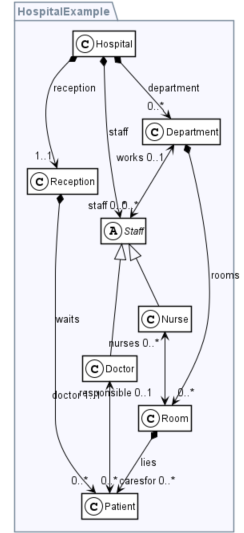
\includegraphics[scale=0.7]{pictures/goal_vis_PlantUML.png}
    \caption{\centering{Goal model in PlantUML}}
    \label{plantUml goal}
\end{figure}

Please also compare your \textbf{Multiplicities}, \textbf{attributes}, \textbf{default literal values}, \textbf{containment values} and all \textbf{names} to fig \ref{goal model}. Differences can result in errors later on.\newline

Congratulations on completing the first part of this tutorial!

\clearpage
